\documentclass[a4paper, 12pt]{article}
\usepackage{graphicx}
\usepackage{caption}
\usepackage{cmap}
\usepackage{tikz}
\usepackage[utf8]{inputenc}
\usepackage[english]{babel}
\usepackage{amsmath, amsfonts, amssymb, amsthm, mathtools}

\title{}
\date{}

%-----------------------------------СOLONTITLE--------------------------------------------

\usepackage{fancyhdr}

   \pagestyle{fancy}
   \fancyhead{}
   \fancyhead[L]{differentiator}
   \fancyhead[R]{Groshev Maxim}
   \fancyfoot[C]{\thepage}

%-------------------------------------------------------------------------------------------
\usepackage{extsizes}
\begin{document}

%-----------------------------------TITLEPAGE-----------------------------------------------

    \begin{titlepage}
    \maketitle
    \thispagestyle{empty}

            \begin{center}
                  \Large \textbf{DIFFERENTIATOR}
            \end{center}

             \vspace{20em}
             \begin{flushright}
                 \normalsize Made by: \\
                             Groshev M. B01-206
             \end{flushright}

             \begin{center}
                    \vfill \normalsize Dolgoprudniy \\ 2023
             \end{center}
    \end{titlepage}


\section{I am here to find you and I will...}\begin{equation*}
    f = ({{120}}+{\cos({\ln({{x}})})})
\end{equation*}

\begin{figure}[h!]
        \centering
         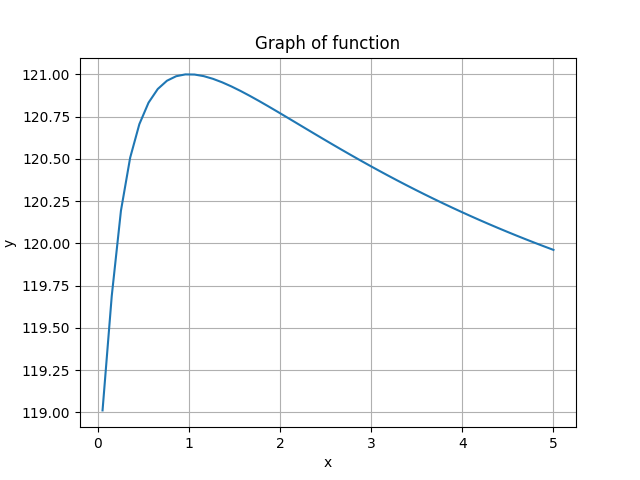
\includegraphics[scale=0.5]{./LaTeX/tex_pics/func.png}
\end{figure}

\section{I did it... But at what cost}\begin{equation*}
    \frac{d}{dx} = ({{0}}+{{{{-1}}\cdot{\sin({\ln({{x}})})}}\cdot{{\frac{{1}}{{x}}}\cdot{{1}}}})
\end{equation*}

\section{The final trivial transition}\begin{equation*}
    \frac{d}{dx} = {{{-1}}\cdot{\sin({\ln({{x}})})}}\cdot{\frac{{1}}{{x}}}
\end{equation*}

\begin{figure}[h!]
        \centering
         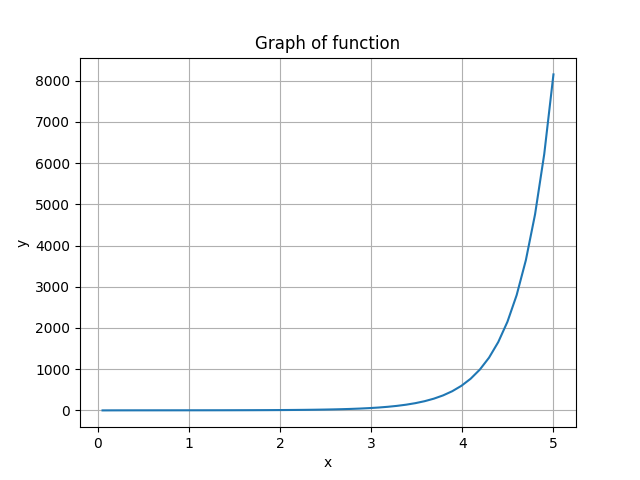
\includegraphics[scale=0.5]{./LaTeX/tex_pics/differ.png}
\end{figure}

\end {document}